\documentclass[authoryear,review,12pt]{elsarticle}
%\usepackage{amsmath,lineno,fullpage}
%\usepackage{lineno}
\begin{document}
%\linenumbers
%\pagestyle{empty}
%\doublespace
\begin{frontmatter}
\journal{Quaternary Geochronology}
\title{Interlaboratory comparison of cosmogenic $^{21}$Ne in quartz}
\author[eth,ucl]{Pieter Vermeesch}
\author[bgc]{Greg Balco}
\author[crpg]{Pierre-Henri Blard}
\author[koln]{Tibor J. Dunai}
\author[eth]{Florian Kober} 
\author[gfz]{Samuel Niedermann}
\author[ucb,bgc]{David L. Shuster}
\author[eth]{Stefan Strasky}
\author[suerc]{Finlay M. Stuart}
\author[eth]{Rainer Wieler}
\author[crpg]{Laurent Zimmermann}
\address[eth]{Institute of Geochemistry and Petrology, ETH Zurich, Z\"{u}rich, Switzerland}
\address[ucl]{London Geochronology Centre, University College London, London, United Kingdom}
\address[bgc]{Berkeley Geochronology Center, Berkeley, United States}
\address[ucb]{Department of Earth and Planetary Science, University of California, Berkeley, United States}
\address[crpg]{Centre de Recherches P\'{e}trologiques et G\'{e}ochimiques, Vandoeuvre-l\`{e}s-Nancy, France}
\address[koln]{University of Cologne, K\"{o}ln, Germany}
\address[gfz]{Deutsches GeoForschungsZentrum GFZ, Potsdam, Germany}
\address[suerc]{Scottish Universities Environmental Research Centre, Glasgow, United Kingdom}

\begin{abstract}
We performed an interlaboratory comparison study with the aim to
determine the accuracy of cosmogenic $^{21}$Ne measurements in quartz.
CREU-1 is a natural quartz standard prepared from amalgamated vein
clasts which were crushed, thoroughly mixed, and sieved into 125-250
$\mu$m and 250-500$\mu$m size fractions.  50 aliquots of CREU-1 were
analyzed by five laboratories employing six different noble gas mass
spectrometers.  The released gas contained a mixture of 16-30\%
atmospheric and 70-84\% non-atmospheric (predominantly cosmogenic)
$^{21}$Ne, defining a linear array on the
$^{22}$Ne/$^{20}$Ne-$^{21}$Ne/$^{20}$Ne three isotope diagram with a
slope of 1.108$\pm$0.014.  The internal reproducibility of the
measurements is in good agreement with the formal analytical
precision for all participating labs.  The external reproducibility of
the $^{21}$Ne concentrations between labs, however, is significantly
overdispersed with respect to the reported analytical precision.  We
report an average reference concentration for CREU-1 of
348$\pm$10$\times$10$^6$at[$^{21}$Ne]/g[SiO$_2$], and suggest that the
7.1\% (2$\sigma$) overdispersion of our measurements may be
representative of the current accuracy of cosmogenic $^{21}$Ne in
quartz.  CREU-1 was tied to CRONUS-A, which is a second reference
material prepared from a sample of Antarctic sandstone.  We propose a
reference value of 320$\pm$11$\times$10$^6$at/g for CRONUS-A.  The
CREU-1 and CRONUS-A intercalibration materials may be used to improve
the consistency of cosmogenic $^{21}Ne$ to the level of the analytical
precision.
\end{abstract}
\end{frontmatter}

\section{Introduction}
Cosmogenic neon is a relatively little used tool for studying Earth
surface processes. It is powerful for four reasons.  First, it is
produced and retained in quartz \citep{niedermann1993, niedermann1994,
  shuster2005b} as well as most other silicates, such as pyroxene
\citep{schaefer1999}, olivine \citep{poreda1992}, sanidine
\citep{kober2005}, hornblende and biotite
\citep{amidon2012}. Therefore, it is applicable to most rock types
found on the Earth's surface.  Second, cosmogenic $^{21}$Ne is a
stable nuclide. This gives it an age range limited essentially only by
the erosion rate and allows exceptionally old landscapes to be dated
\citep{schaefer1999, dunai2005}.  Third, neon has three isotopes
($^{20}$Ne, $^{21}$Ne, and $^{22}$Ne), each of which have different
abundances in the various reservoirs (atmospheric, nucleogenic, or
magmatic) that may contribute to the natural $^{21}$Ne background
\citep{niedermann2002}.  By simultaneously analyzing all three
isotopes and verifying whether they plot on a mixing line between
atmospheric and spallogenic components, the cosmogenic neon method
provides an internal `reliability check' which is absent from other
commonly used nuclides. Fourth, neon can be measured using a standard
sector field noble gas mass spectrometer. Sample requirements are
modest (typically 100-200 mg) and sample preparation is relatively
straightforward as it does not require extensive chemical purification
or chromatography. This greatly increases sample throughput, which in
turn opens up exciting opportunities for detrital work
\citep{dunai2005, codilean2008}.\\

Cosmogenic $^{21}$Ne is even more useful when combined with one or
more cosmogenic radionuclides such as $^{10}$Be or $^{26}$Al. Such
double- or triple-dating may be used for burial dating
\citep{balco2009b, vermeesch2010b}, for catchment-wide erosion studies
with complex exposure histories \citep{kober2009}, or to measure the
exposure age of old and very slowly eroding surfaces
\citep{fujioka2005}. An implicit assumption of many of these studies
is that the accuracy of the $^{21}$Ne method equals its analytical
precision.  Violation of this assumption may lead to erroneous results
such as samples plotting in the `forbidden zone' of the
$^{21}$Ne/$^{10}$Be two-nuclide diagram \citep{lal1991, kober2011}. An
interlaboratory comparison study was set up in the framework of the
CRONUS-EU initiative \citep{stuart2009} with the aim to address this
issue and provide the noble gas community with a well-characterized
reference standard for the analysis of cosmogenic $^{21}$Ne in
quartz. The CREU-1 standard is a mixture of natural quartz pebbles,
rich in cosmogenic $^{21}$Ne, which were crushed and thoroughly
homogenized to ensure optimal reproducibility (Section
\ref{sec:sampleprep}).  Two size-fractions of CREU-1 were analyzed by
five prominent cosmogenic noble gas laboratories, each of which used
different experimental setups and data reduction protocols (Section
\ref{sec:methods}). In total, 50 aliquots of CREU-1 were analyzed,
with reported analytical precisions of 2-6\%, but an external
reproducibility of 7.1\% (Section \ref{sec:results}). These analyses
were tied to a further 10 measurements of CRONUS-A, which is a second
reference material prepared from an Antarctic quartzite analysed by
two of the participating labs (Section \ref{sec:cronus-a}).

\section{Standard material}
\label{sec:sampleprep}

The CREU-1 standard material is pure quartz prepared from exposed
vein-quartz clasts of a Miocene erosion surface
(19$^{\circ}$33'53.4''S, 70$^{\circ}$7'1.5''W, 930 m) in the Atacama
desert near Pisagua, Chile \citep[between sites B and C
  of][]{dunai2005}.  The clasts were shed onto the surface from local
sources after the main sedimentation episode at $\sim$12-14 Ma
\citep{dunai2005}.  Approximately 400g of material was mixed from five
clasts (sample name CH04/5, pebbles 5, 6, 7, 8 and 13, weighing 81g,
104g, 77g, 109g and 55g respectively) that had $^{21}$Ne excess
concentrations within 5\% of their mean value. After crushing in a
W-carbide disk mill, five size fractions were prepared using stainless
steel sieves:

\begin{itemize}
\item 40-62$\mu$m: 10.45g, wet sieved and dried overnight at 50$^{\circ}$C
\item 63-125$\mu$m: 40.62g, wet sieved and dried overnight at 50$^{\circ}$C
\item 125-250$\mu$m: 74.4g, dry sieved
\item 250-500$\mu$m: 188g, dry sieved
\item $>$500$\mu$m: 15.8g, dry sieved
\end{itemize}

Of these five fractions, the 125-250$\mu$m and 250-500$\mu$m fractions
were taken to produce the standard material, while the remaining
fractions were preserved, but not processed any further.  The
125-250$\mu$m and 250-500$\mu$m fractions were soaked in concentrated
sulfuric acid at 120$^{\circ}$C overnight, to remove all iron coatings
and accessory minerals such as rutile, sphene and fluorite. After the
acid treatment, the material was rinsed ten times in cold de-ionized
water, followed by five times one hour ultrasonic rinsing in
de-ionized water at 80$^{\circ}$C.  Next, the quartz was dried
overnight at 110$^{\circ}$C. Although the preparation steps outlined
above probably already ensured a thoroughly mixed quartz sand, a
FRITSCH$^{\tiny\textregistered}$ rotary cone sample divider laborette
27 was used to split the material into 16 equal fractions. Different
aliquots of CREU-1 have been analyzed by five noble gas laboratories,
at BGC (Berkeley), CRPG (Nancy), ETH (Z\"{u}rich), GFZ (Potsdam) and
SUERC (Glasgow).

\section{Analytical methods}
\label{sec:methods}

The five participating laboratories employed a variety of noble gas
mass spectrometers and analytical procedures for cosmogenic $^{21}$Ne
analysis. Rather than forcing all the participants to use the same
heating schedules, gettering times and so forth, they were allowed to
use their own measurement routines, so that the calibration exercise
fully captured the diversity of approaches used for $^{21}$Ne
analysis. The temperature steps and amount of material used are
reported in Tables 1-3.

\subsection{BGC}

Neon extraction from quartz at BGC employed a 14-sample vacuum chamber
with a 3 inch diameter sapphire viewport. Samples of up to 150 mg
quartz were encapsulated in a Ta packet and heated through the
viewport by a 150 W diode laser ($\lambda$ = 810 nm) using a feedback
control system in which the temperature of the packet was continuously
monitored by an optical pyrometer coaxial with the laser delivery
optic. Calibration of the pyrometer for the emissivity of the Ta
packets was accomplished by placing a thermocouple in the same
apparatus. Collateral heating of adjacent samples was prevented by
completing one heating step for all samples before beginning the next
heating step. This procedure was tested by interspersing blanks
consisting of an empty Ta packet. After heating, sample gas was
reacted with a SAES$^{\tiny\textregistered}$ getter and adsorbed to a
cryogenic trap at 20 K. Neon was then released into the mass
spectrometer at 70 K. All sample heating, gas processing, and
measurement operations were automatically controlled.  Analyses were
done with a MAP-215 mass spectrometer updated with modern ion-counting
electronics. Under normal operating conditions, this machine had a
relatively low Ar$^{+}$/Ar$^{++}$ ratio (2.5-5, depending on source
tuning) and inadequate mass resolution to fully resolve
$^{20}$Ne$^{+}$ from $^{40}$Ar$^{++}$, so a correction for background
$^{40}$Ar$^{++}$ was required. As described in \citet{balco2009a},
this was accomplished by introducing a $^{39}$Ar spike and monitoring
the Ar charge ratio as well as the $^{40}$Ar$^{+}$ signal throughout
each analysis.  The resulting correction on mass 20 varied between
analyses, but was typically equivalent to
5.00$\pm$0.02$\times$10$^{8}$ atoms $^{20}$Ne.  Similarly, a
correction for $^{12}$C$^{16}$O$_{2}^{++}$ on mass 22 was made by
establishing a relationship between the Ar and CO$_{2}$ charge ratios.
Absolute calibration of Ne abundance was made by peak height
comparison against an air standard processed in the same way as the
samples and analyzed several times daily.  Linearity of machine
response was verified by varying the volume of the air standard.  The
pressure of the air standard reservoir was measured during loading
with an MKS Baratron manometer, and corrected for atmospheric water
vapor using three separate hygrometers at the time of air sample
collection.  Absolute volumes of the reservoir and pipette were
determined by differential pressure measurements, again using the
Baratron, against two separate reference glass ampules whose volumes
were independently measured by Hg weighing. The amount of cosmogenic
$^{21}$Ne was calculated by assuming two-component mixing of
atmospheric and cosmogenic neon.  Reported uncertainties include i)
counting uncertainties on all masses, including those used to generate
corrections for $^{40}$Ar$^{++}$ and CO$_{2}^{++}$; ii) uncertainty in
blank subtraction (the $^{21}$Ne process blank was $\sim$ 0.5 Hz or
$\sim$ 90,000 atoms, which was $<$ 1\% of typical signals on mass 21
for these measurements); and iii) the reproducibility of the air
standards ($\sim$1\% for $^{20}$Ne, $\sim$3\% for $^{21}$Ne).

\subsection{CRPG}

After 10 minutes cleaning in an acetone ultrasonic bath, quartz
aliquots were wrapped in copper foils (Alfa
Aesar$^{\tiny\textregistered}$, 0.025 mm thick, 99.8\%). Samples were
then loaded under high vacuum in a stainless steel carousel that had
been baked during 10 h at 80$^{\circ}$C. Gas extraction from the
quartz was realized by 25 minutes heating in a home-designed single
vacuum resistance furnace with a boron nitride crucible
\citep{zimmermann2012}. Sequential purification with charcoals in
liquid nitrogen, titanium sponges
(Johnson\-Matthey$^{\tiny\textregistered}$, mesh m3N8 t2N8) and
SAES$^{\tiny\textregistered}$ getters (ST172/HI/20-10/650C) permitted
gas cleaning by removal of H$_2$O, Ar, Kr, Xe and hydrocarbons. Ne was
not separated from He. The purified gas was finally analyzed using a
VG5400 mass spectrometer. Corrections for isobaric interferences of
$^{40}$Ar$^{++}$ at m/e = 20 and $^{12}$C$^{16}$O$_2^{++}$ at m/e = 22
were negligible compared to the amount of analyzed neon. The mass
spectrometer sensitivity was determined by peak height comparison
against a 0.2 cm$^3$ ($\sim$1.6$\times$10$^{10}$ atoms of $^{20}$Ne)
pipette of a gas standard having an atmospheric composition. Typical
furnace blanks at 1000-1300$^\circ$C (25 min) were
1.0$\pm$0.2$\times$10$^{8}$, 3$\pm$1$\times$10$^{5}$ and
1.63$\pm$0.06$\times$10$^{7}$ atoms of $^{20}$Ne, $^{21}$Ne and
$^{22}$Ne, respectively. Excess $^{21}$Ne ($^{21}$Ne$^*$)
concentrations were calculated following:

\begin{equation}
^{21}Ne^* = R_c \times ^{20}Ne_m \times (R_m-R_a) / (R_c-R_a) 
\label{eq:Blard}
\end{equation}

where $^{20}$Ne$_m$ is the measured $^{20}$Ne, R$_c$ is the cosmogenic
$^{21}$Ne/$^{20}$Ne-ratio \citep[R$_c$ = 0.8;][]{niedermann2002},
R$_m$ is the measured $^{21}$Ne/$^{20}$Ne-ratio, and R$_a$ is the
atmospheric $^{21}$Ne/$^{20}$Ne-ratio (R$_a$ = 0.00296).

\subsection{ETH}

Noble gases were extracted by heating in a molybdenum crucible.
Released gases were cleaned in a stainless steel extraction line
equipped with Al/Zr-getters (SAES$^{\tiny\textregistered}$) and
activated charcoal held at the temperature of liquid nitrogen before
He and Ne were expanded to a cryogenic pump. Helium and neon were
separated by adsorbing neon at 14 K on stainless steel frits and
analyzing helium first.  After pumping away the helium, neon was
released from the cryotrap at 50 K.  Noble gas analyses were performed
in a custom-made, all-metal magnetic sector mass-spectrometer
(90$^{\circ}$, 210 mm radius) equipped with a modified Baur-Signer ion
source with essentially constant sensitivity over the pressure range
relevant for this work \citep{baur1980}.  The ion source was equipped
with a compressor device increasing the sensitivity by factors of 120
and 200 for $^3$He and $^{21}$Ne, respectively \citep{baur1999}
compared to the sensitivities of the same spectrometer with the
compressor turned off.  The absolute sensitivity and mass
discrimination of the mass spectrometer were determined by analysing
known amounts of standard noble gas mixtures prepared from
commercially available pure gases. The Ne isotopic composition of the
standard gas was cross calibrated against two air standards
\citep{heber2009}. Similarly, the Ne amounts delivered by the standard
pipette were cross calibrated with air standards as well as with other
independently filled standard gas bottles. The uncertainty of the Ne
standard gas amounts is estimated to be 2\% \citep{heber2009}.  Full
procedural blanks (45' at 600$^{o}$C + 20' at 800$^{\circ}$ + 15' at
1750$^{\circ}$C) were 1.211$\pm$0.006$\times$10$^{8}$,
3.5$\pm$0.2$\times$10$^{5}$, and 1.17$\pm$0.01$\times$10$^{7}$ atoms
of $^{20}$Ne, $^{21}$Ne and $^{22}$Ne, respectively.  Corrections for
isobaric interferences on mass 20 have been applied for
$^{40}$Ar$^{++}$ and H$_2^{18}$O$^+$ but were always less than 2\%.
No correction for CO$_2^{++}$ on $^{22}$Ne was necessary.  The low
correction factors for doubly charged species were the results of a
low electron acceleration voltage of 45V in the ion source. Excess
$^{21}$Ne ($^{21}$Ne$^*$) concentrations were calculated with Equation
\ref{eq:Blard}.

\subsection{GFZ}

CREU-1 quartz samples were wrapped in aluminium foil and loaded in a
sample carousel without further treatment, except for two aliquots of
the 250-500$\mu$m fraction (GFZ-6-7) which were crushed to
$\sim$50$\mu$m grain size in an agate mortar before loading.  Noble
gases were extracted in a resistance-heated furnace equipped with a
tantalum crucible and molybdenum liner and analyzed in either of two
VG5400 noble gas mass spectrometers, with measurements GFZ1-7 being
measured on one machine, and GFZ8-11 on the other (Tables 1 and 2).
GFZ-8 was not heated, but instead crushed in vacuo between two hard
metal jaws in order to test whether Ne trapped in fluid inclusions of
CREU-1 has an atmospheric isotopic composition.  Gas purification
involved a dry ice trap, two titanium sponge and foil getters, and two
SAES$^{\tiny\textregistered}$ (Zr-Al) getters.  The noble gases were
trapped on stainless steel frits and/or activated charcoal in
cryogenic adsorbers and sequentially released for He, Ne, and Ar-Kr-Xe
analysis. Isobaric interferences of $^{40}$Ar$^{++}$ at m/e=20 (up to
20\% at 400$^{\circ}$C) and $^{12}$C$^{16}$O$_2^{++}$ at m/e=22 (up to
10\% at 400$^\circ$C) were corrected according to the method described
by \citet{niedermann1993, niedermann1997}. A correction for
H$_2^{18}$O$^+$ at m/e=20 was not necessary due to the mass resolution
of $\geq$600.  Blanks had an atmospheric composition and contained
1-3$\times10^{7}$ atoms of $^{20}$Ne, depending on temperature.
Excess $^{21}$Ne was calculated without applying a blank correction,
assuming an atmospheric origin of all the measured $^{20}$Ne:

\begin{equation}
^{21}Ne^* = ^{21}Ne_m \times (R_m - R_a) / R_m
\label{eq:GFZ}
\end{equation}

with all abbreviations as in Equation \ref{eq:Blard}.  In some cases a
high atmospheric Ne memory (i.e., rapid decay of non-atmospheric Ne
isotope ratios) required the application of a special procedure to
derive the Ne concentration and isotopic composition at the time of
gas admission to the mass spectrometer
\citep[see][]{goethals2009b}. Absolute noble gas concentrations were
obtained by peak height comparison against a 0.1 cm$^3$ pipette of
calibration gas \citep[an artificial mixture of the five noble gases
  in nitrogen provided by Linde company;][]{niedermann1997}, which was
cross-calibrated in the 1990s against glass ampoule noble gas
standards made available by O.  Eugster (University of Bern) and whose
noble gas concentrations are judged accurate to $\sim$3\% at 95\%
confidence level, and have been propagated into the overall
uncertainty.

\subsection{SUERC}

The clean quartz was thoroughly rinsed in ultra-pure acetone and
packed into aluminium foil cylinders.  Cosmogenic Ne was extracted by
heating each sample packet for 20 minutes. The active gases were
removed by exposure to two hot SAES$^{\tiny\textregistered}$ (Zr-Al)
getters during heating, and for a further 20 minutes as the furnace
cooled. The heavy noble gases and residual active gases were
subsequently adsorbed on liquid nitrogen cooled activated charcoal for
10 minutes and exposed to a getter at room temperature to adsorb
hydrogen. Neon was then adsorbed on activated charcoal in a cryostatic
cold head at 30K. The helium was pumped for 1 minute, then the Ne was
desorbed from the charcoal trap at 100K.  Neon isotopes were analyzed
statically in a MAP-215 magnetic sector mass spectrometer equipped
with a modified Nier-type ion source, an axial electron multiplier
(Burle Channeltron) operated in pulse-counting mode and a Faraday
detector. A room temperature SAES$^{\tiny\textregistered}$ G50 getter
and a liquid nitrogen-cooled activated charcoal trap were used to
minimize the contribution of interfering species during analysis. The
data presented here were taken over a period of two
years. Consequently source conditions changed to a small
degree. Typically the source was tuned for Ne sensitivity prior to
analytical periods; electron voltage of 88 V, trap current of 500
$\mu$A and an acceleration voltage of 3 kV. A slit in front of the
electron multiplier was used to achieve a resolving power
(m/$\Delta$m) of approximately 400. For all samples and calibrations
the abundances of masses 18, 19, 20, 21, 22, 40 and 44 were determined
by integrating counts recorded in 40-100 blocks of 5 seconds
each. Peak heights of masses 2 and 16 were measured on the Faraday
detector.  Instrumental sensitivity was calculated from repeated
analysis of aliquots of 2.2$\times$10$^{10}$ atoms $^{20}$Ne in air
sampled from a 5 liter reservoir. Isotopic mass discrimination was
approximately 0.50 $\pm$ 0.03 \%/amu. The average high temperature
$^{20}$Ne blank was 1$\times$10$^8$ atoms. There was no observed
increase when empty Al foil was heated. The Ne isotopic composition of
blank measurements after correction for interfering species (see
below) was indistinguishable from air ratios. Since it is likely that
a significant amount of air-derived Ne is released from the quartz
during heating, no blank correction has been made to the data.  Excess
$^{21}$Ne concentrations were calculated assuming an atmospheric
origin of all the measured $^{20}$Ne according to Equation
\ref{eq:GFZ}.  Interference at m/e = 20 from H$_2^{18}$O$^+$ was
calculated from measurement of H$_2^{16}$O$^+$ at mass 18. The
contribution never exceeded 0.03\%. No H$^{19}$F$^+$ signal was
observed in blanks and mass spectrometer backgrounds. The dominant
interference at m/e = 20 came from $^{40}$Ar$^{++}$. The charge state
ratio $^{40}$Ar$^+$/$^{40}$Ar$^{++}$ is governed by the partial
pressure of H in the mass spectrometer ionization region. A
first-order relationship between $^{40}$Ar$^+$/$^{40}$Ar$^{++}$ and
H$^+$ beam size was recorded.  The partial pressure of H remained
constant resulting in $^{40}$Ar$^+$/$^{40}$Ar$^{++}$ = 2.30-2.32. The
contribution of $^{40}$Ar$^{++}$ to the measured $^{20}$Ne signal in
CREU quartz samples was $<$1\%.  Correction for
$^{12}$C$^{16}$O$_2^{++}$ at m/e = 22 was calculated from measured
mass 44 ($^{12}$C$^{16}$O$_2^{+}$) using a CO$_2^{+}$/CO$_2^{++}$ = 50
to 58 (determined by repeated measurements interspersed with sample
measurements). No pressure dependence on the CO$_2^+$/CO$_2^{++}$
ratio was recorded for a 50-fold variation in the partial pressure of
H and CO$_2$. Correction for interfering $^{12}$C$^{16}$O$_2^{++}$
never exceeded 1\%.

\section{Results}
\label{sec:results}

\begin{figure}
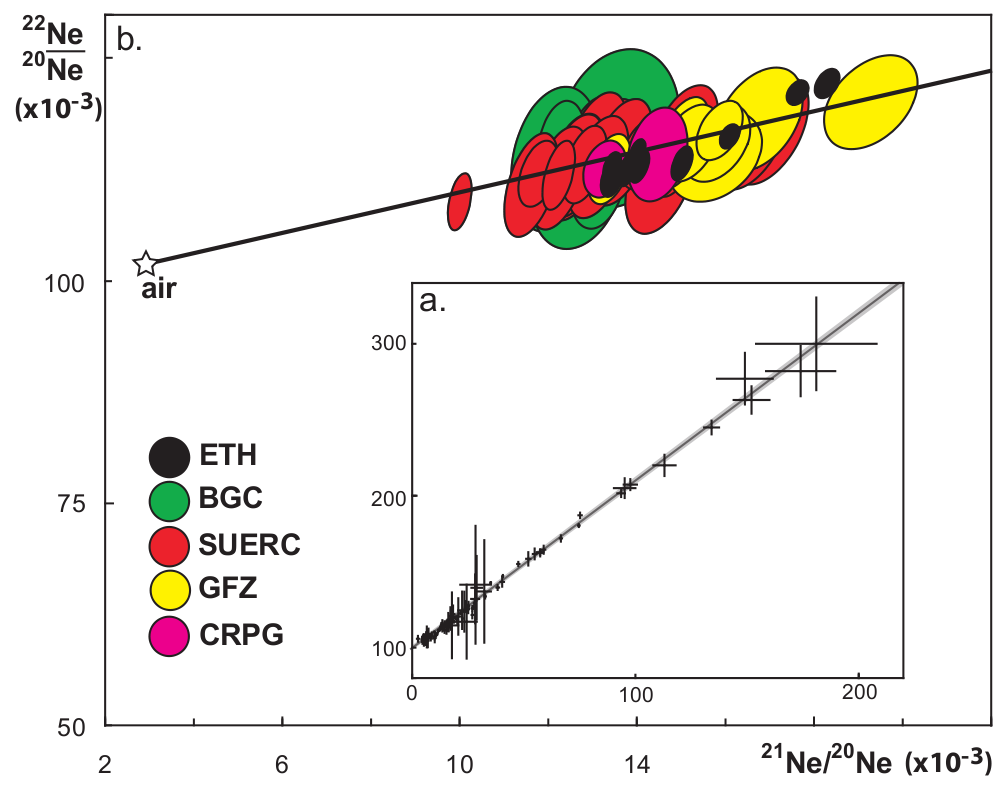
\includegraphics[width=500pt]{Figure1.png}
\caption{Neon three-isotope plots of (a) all the individual heating
  steps and (b) the total released gas for each analyzed CREU-1
  aliquot.  The data fit a spallation line with a slope of 1.108 $\pm$
  0.014 (2$\sigma$, MSWD = 3.4). Error symbols are 1$\sigma$.}
\label{fig:3-isotope}
\end{figure}

All five labs reported data for the coarse fraction, while three labs
measured the fine fraction as well. The results for both sets of
analyses are reported in Tables 1 and 2.
The $^{21}$Ne/$^{20}$Ne and $^{22}$Ne/$^{20}$Ne compositions of the
individual heating steps and their sums are consistent with a
predominantly spallogenic origin of the released $^{21}$Ne (Figure
1). The pooled analyses comprise 16-30\% atmospheric
and 70-84\% excess $^{21}$Ne, with individual heating steps containing
up to 98\% excess $^{21}$Ne.  Linear regression of the spallation line
yields a slope of 1.108 $\pm$ 0.014 (2$\sigma$), which is in
statistical agreement with previously published values \citep[Table 8
  of][]{niedermann2002}.  \\

The total excess $^{21}$Ne contents of all the aliquots are shown in
Figure 2.  The reported 2$\sigma$ analytical uncertainties are between
2 and 6\%. The MSWD \citep[Mean Square of the Weighted Deviates,
  a.k.a. `reduced Chi-square',][]{mcintyre1966} is reasonably close to
unity for ETH, GFZ and BGC, indicating good agreement of the observed
scatter with the measurement errors. The extremely low MSWD of 0.005
for CRPG may indicate overestimated analytical uncertainties, but
could also be due to chance, as only two aliquots were
analyzed. Finally, the coarse fraction of SUERC is characterized by an
MSWD of 4.1, which may indicate underestimated analytical
uncertainties. However, measurements of the fine fraction by the same
lab have an MSWD of 1.3. There is no systematic difference between the
fine and the coarse grain size fractions of ETH, SUERC and GFZ.
Measurements GFZ-6-7 were performed on material from the coarse
fraction that was crushed for 5 minutes in air with an agate mortar to
$\sim$50$\mu$m, resulting in some loss of excess $^{21}$Ne.  GFZ-8 was
crushed in vacuo, and the data shown are for that crushing extraction.
The $^{21}$Ne excess of GFZ-8 is considerably less than the $^{21}$Ne
deficit in GFZ-6-7, probably because the in-vacuo crusher was much
less efficient than the mortar.  Measurements GFZ-6-8 were not
included in subsequent calculations and figures.  Total $^3$He
concentrations measured at GFZ were 204$\pm$10$\times$10$^6$at/g for
the coarse fraction (seven measurements) and
109$\pm$7$\times$10$^6$at/g (a single analysis) for the fine
fraction. The resulting $^{21}Ne/^3He$-ratios are significantly
greater than the production-rate ratio. This is likely caused by a
combination of helium loss due to hot acid etching during sample
preparation, and the fact that helium is not quantitatively retained
in quartz at surface temperatures \citep{shuster2005b}.\\

BGC analyzed material from two different vials of CREU-1, thus
presenting an opportunity to verify the homogeneity of the
standard. Measurements BGC-1-4 were performed on material from the same
vial as ETH, whereas measurements BGC-5-8 were done on the same vial as
CRPG.  The observed difference between the two vials analyzed by BGC
falls within the analytical uncertainty. The difference between the
results of BGC and ETH/CRPG, however, falls well outside the
statistically acceptable range.  The error-weighted means of all the
labs do not agree with each other within the analytical uncertainties,
defined as the standard errors of those means. Therefore, in order to
calculate a global average of all the data (using both the fine and
the coarse grain fractions), we used a random effects model with two
sources of uncertainty. We assume that the intra-laboratory averages
x$_i$ (where i is an identifier for each participating lab) come from
a normal distribution of the form:

\begin{equation}
x_i \sim N(\mu,\sigma_i^2 + \zeta^2)
\label{eq:overdispersion}
\end{equation}
 
where $\mu$ is the global mean, $\sigma_i^2$ the analytical
uncertainty (variance) of the i$^{th}$ lab, and $\zeta^2$ is the
amount of {\it overdispersion}, i.e. the excess scatter (variance)
that cannot be explained by the analytical uncertainty alone.  To
understand this formula, consider the following two special cases.  If
$\sigma_i=0$ (perfect reproducibility within each lab) then $\mu$ is
the arithmetic mean of the laboratory averages.  And if $\zeta=0$
(perfect reproducibility between all labs) then $\mu$ is the
error-weighted mean of those same laboratory averages.  In order to
simultaneously take into account the finite analytical precision of
each lab and the variance between the labs, Equation
\ref{eq:overdispersion} was iteratively solved for both $\mu$ and
$\zeta$, yielding an average $^{21}$Ne concentration of
348$\pm$10$\times$10$^6$at/g and an overdispersion (defined as
2$\zeta$/$\mu$) of 7.1\%.

\begin{figure}
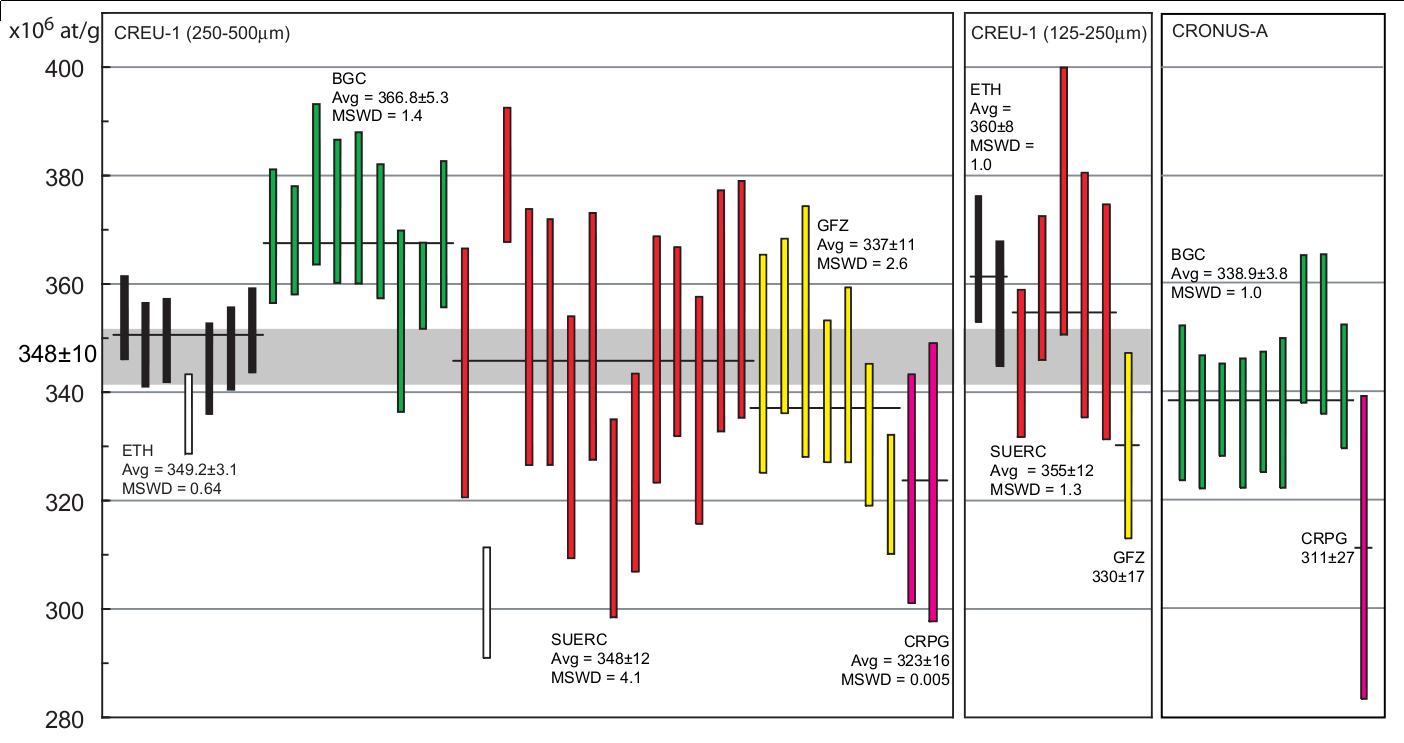
\includegraphics[width=500pt]{Figure2.png}
\caption{Overview of all the reported $^{21}$Ne concentrations and
  2$\sigma$ uncertainties, with indication of the error-weighted means
  for each participating laboratory.  White bars are considered
  outliers and were not used to calculate the averages.  Left and
  middle panels: coarse and fine fractions of CREU-1; right panel:
  CRONUS-A.  Gray band marks the average and 2$\sigma$ uncertainty of
  CREU-1.}
\label{fig:average}
\end{figure}

\section{Comparison with CRONUS-A}
\label{sec:cronus-a}

In addition to CREU-1, two of the participating labs also analyzed
CRONUS-A as a second reference material. CRONUS-A was collected in
Antarctica's Arena Valley (77$^\circ$ 52' 58.9''S, 160$^\circ$ 56'
35.1''E, 1666m elevation), from a large (40kg) yet thin ($\sim$2cm)
slab of Beacon sandstone. Quartz was purified at the University of
Vermont by crushing, sieving and repeated etching in dilute HF, using
procedures designed for cosmogenic $^{10}$Be-$^{26}$Al analysis. CRPG
reported one and BGC a further nine analyses of CRONUS-A, using the
same protocols that were used for the CREU-1 measurements (Table 3).
The average cosmogenic $^{21}$Ne content of the nine CRONUS-A samples
measured by BGC was 338.9$\pm$3.8$\times$10$^6$at/g, i.e.
7.6$\pm$3.7\% lower than that of CREU-1. The single CRONUS-A analysis
of CRPG is lower than its CREU-1 measurements by a similar amount
(4$\pm$17\%), although the reported analytical precision of the latter
estimate is much poorer.  Additionally, published CRONUS-A values have
been reported by two laboratories which did not participate in the
interlaboratory comparison, at Harvard University
\citep[330$\pm$3$\times$10$^6$at/g,][]{middleton2012} and the
California Institute of Technology
\citep[338$\pm$10$\times$10$^{6}$at/g,][]{amidon2012}.  Normalizing
the average CRONUS-A value reported by BGC to the CREU-1 reference
value results in a $^{21}Ne$ concentration of
320$\pm$11$\times$10$^6$at/g. We propose that when this value is used
as a reference, CRONUS-A can serve as an alternative to CREU-1.

\section{Discussion}
\label{sec:discussion}

It is interesting to note that significant amounts of excess $^{21}$Ne
remained trapped in the quartz after the second highest heating step,
at temperatures of up to 820$^\circ$C. Total degassing was not
achieved until the final temperature step at 1140$^\circ$C and
more. This is significantly higher than the 800$^\circ$C release
temperature for cosmogenic neon reported by
\citet{niedermann2002}. Nevertheless, for all samples of all labs, the
data points of the higher temperature steps plot on the mixing line
between atmospheric and cosmogenic neon (Figure 1),
which strongly suggests that the non-atmospheric neon in all samples is
essentially purely cosmogenic, although quartz occasionally also
contains a nucleogenic neon component released at high temperature with
a $^{21}$Ne/$^{22}$Ne ratio of approximately unity
\citep[Ne$_{HT}$,][]{niedermann1994, niedermann2002}. However, in view
of the position of all data points in Figure 1 it
seems very improbable that a sizeable fraction of the non-atmospheric
$^{21}$Ne in our samples could be nucleogenic Ne$_{HT}$. Even in this
unlikely case this would be largely irrelevant for the purpose of
interlaboratory comparison, because for all samples we sum the
non-atmospheric $^{21}$Ne from all temperature steps.\\

Despite the fact that CREU-1 is pure and highly enriched in
spallogenic neon, the $^{21}$Ne concentrations reported by the
participating labs are significantly overdispersed with respect to the
formal analytical uncertainty.  In theory, this overdispersion could
be due to inhomogeneity of the standard material itself, as different
labs analyzed aliquots from different vials of CREU-1. However, the
analysis of two of these vials by BGC, and comparison with
measurements of those same vials by ETH and CRPG, shows that this is
not the case. Therefore, CREU-1 is homogenous.  If the overdispersion
cannot be attributed to the standard material itself, then it must be
due to biases introduced by the different standard calibration bottles
used \citep{heber2009}, or to differences in the neon sensitivity
between samples and standards introduced by sample processing or
tuning conditions.

\section{Conclusion}
\label{sec:conclusion}

Our calibration experiment has shown that, although the reported
analytical precision of cosmogenic noble gas measurements may be as
low as 2\%, the accuracy is not quite as good. We suggest that the
7.1\% dispersion observed in our study be used as a more realistic
estimate of the accuracy of the $^{21}$Ne method at the present
time. It should be borne in mind that this may even be an optimistic
value, for a highly enriched and well behaved standard material. Using
realistic and conservative analytical uncertainties is especially
important for studies combining $^{21}$Ne with other (radio)nuclides,
and to assess the resolving power of such studies. For single nuclide
studies, CREU-1 or CRONUS-A measurements can be used to normalize
$^{21}$Ne to the reference values reported in this paper, so that
measurements from different labs can be compared on an equal footing
and relative differences in $^{21}$Ne can be compared on the level of
the analytical precision \citep{dunai2009}. Those interested in
obtaining aliquots of these standards may contact T. Dunai
(\verb|tdunai@uni-koeln.de|) for CREU-1 or T. Jull
(\verb|jull@email.arizona.edu|) for CRONUS-A.


\section*{Acknowledgments}

This research was funded by CRONUS-EU (Marie Curie RTN project
511927). We would like to thank Mark Kurz and an anonymous reviewer
for positive and constructive feedback on the submitted manuscript.

\begin{table}
\centering
\caption{Summary table of the coarse fraction of CREU-1.  `21/20'
  and `22/20' are the $^{21}Ne/^{20}Ne$ and $^{22}Ne/^{20}Ne$ ratios,
  $^{21}$Ne$^*$ is excess $^{21}$Ne.  Temperatures of ETH-4-7 (marked
  by an asterisk) and SUERC-8-9 (omitted) were set when the crucible
  was really full causing samples to be degassed at positions where
  the temperature was lower than the nominal crucible
  temperature. GFZ-6-7 were crushed to small grain size
  ($\sim$50$\mu$m) before loading, while GFZ-8 was degassed by in
  vacuo crushing instead of heating. These samples were not included
  in Figures \ref{fig:3-isotope} and \ref{fig:average}.}
\label{tab:coarse}
   \begin{tabular}{|r|rrrrrrrrrrrr|}
\hline
          & mass  & T     & $^{20}$Ne  & 2$\sigma$    & 21/20 & 2$\sigma$    & 22/20 & 2$\sigma$    & $^{21}$Ne* & 
2$\sigma$    & sum   & 2$\sigma$ \\ 
          & [mg]    & [$^\circ$C]   & [$\times$10$^9$at/g] & & [$\times$10$^{-3}$] & 
 & [$\times$10$^{-3}$] & & [$\times$10$^6$at/g] & & 
[$\times$10$^6$at/g] & \\ 
\hline
    ETH-1 & 66.37 & 600   & 13.37 & 0.27  & 24.23 & 0.15  & 126.61 & 0.83  & 285.5 & 6.1   &       &  \\
    \hline
          &       & 800   & 9.85  & 0.20  & 6.96  & 0.11  & 105.59 & 0.67  & 39.6  & 1.0   &       &  \\
          &       & 1750  & 8.70  & 0.19  & 6.22  & 0.10  & 106.57 & 1.00  & 28.4  & 0.8   & 353.5 & 7.6 \\
    ETH-2 & 66    & 600   & 11.45 & 0.24  & 27.78 & 0.26  & 129.17 & 0.74  & 285.1 & 6.5   &       &  \\
          &       & 800   & 8.42  & 0.17  & 7.52  & 0.13  & 106.92 & 1.30  & 38.6  & 1.0   &       &  \\
          &       & 1750  & 6.62  & 0.18  & 6.70  & 0.14  & 105.90 & 0.98  & 24.9  & 0.8   & 348.5 & 7.7 \\
    ETH-3 & 49.23 & 800   & 22.13 & 0.45  & 17.15 & 0.13  & 117.11 & 0.29  & 315.3 & 6.9   &       &  \\
          &       & 1750  & 11.16 & 0.22  & 5.99  & 0.12  & 104.81 & 1.15  & 34.0  & 0.9   & 349.2 & 7.6 \\
          &       &       &       &       &       &       &       &       &       &       &       &  \\
    ETH-4 & 82.13 & 600*  & 1.34  & 0.03  & 74.66 & 0.76  & 180.3 & 1.9   & 96.3  & 2.4   &       &  \\
          &       & 800*  & 1.39  & 0.15  & 26.91 & 0.56  & 125.9 & 3.1   & 33.4  & 3.6   &       &  \\
          &       & 1750* & 25.18 & 0.50  & 11.16 & 0.11  & 109.0 & 1.2   & 207.3 & 4.7   & 335.8 & 7.3 \\
    ETH-5 & 48.56 & 600*  & 1.89  & 0.04  & 47.5  & 1.0   & 155.0 & 2.7   & 84.7  & 2.6   &       &  \\
          &       & 800*  & 1.58  & 0.28  & 22.44 & 0.42  & 119.2 & 2.3   & 30.9  & 5.5   &       &  \\
          &       & 1750* & 29.42 & 0.59  & 10.74 & 0.17  & 108.4 & 1.8   & 229.8 & 5.8   & 344.2 & 8.3 \\
    ETH-6 & 48.73 & 600*  & 1.43  & 0.03  & 66.6  & 1.0   & 171.9 & 4.2   & 91.5  & 2.6   &       &  \\
          &       & 800*  & 2.21  & 0.15  & 24.18 & 0.55  & 124.2 & 1.7   & 47.1  & 3.3   &       &  \\
          &       & 1750* & 28.54 & 0.57  & 10.31 & 0.10  & 108.6 & 1.0   & 210.5 & 4.7   & 347.8 & 7.6 \\
    ETH-7 & 81.3  & 600*  & 1.39  & 0.03  & 75.2  & 1.5   & 187.1 & 3.5   & 100.8 & 3.0   &       &  \\
          &       & 800*  & 1.75  & 0.13  & 27.37 & 0.42  & 126.4 & 2.1   & 42.8  & 3.3   &       &  \\
          &       & 1750* & 28.56 & 0.57  & 10.24 & 0.09  & 108.5 & 0.7   & 208.8 & 4.5   & 351.2 & 7.7 \\
          &       &       &       &       &       &       &       &       &       &       &       &  \\
    BGC-1 & 109.9 & 370   & 4.1   & 1.5   & 24.4  & 9.1   & 117   & 49    & 86.9  & 6.0   &       &  \\
          &       & 740   & 14.0  & 0.9   & 17.3  & 1.2   & 119   & 11    & 200.0 & 7.7   &       &  \\
          &       & 1140  & 20.3  & 1.3   & 7.0   & 0.5   & 105   & 8     & 81.5  & 7.4   & 368   & 12 \\
    BGC-2 & 129.4 & 370   & 5.3   & 0.8   & 22.4  & 3.6   & 125   & 25    & 101.6 & 5.2   &       &  \\
          &       & 740   & 15.0  & 0.5   & 15.9  & 0.6   & 114   & 7     & 194.9 & 7.4   &       &  \\
          &       & 1140  & 19.0  & 0.6   & 6.8   & 0.3   & 105   & 5     & 71.1  & 4.2   & 368   & 10 \\
    BGC-3 & 115.7 & 390   & 4.7   & 0.6   & 28.2  & 3.6   & 132   & 32    & 121.3 & 6.9   &       &  \\
          &       & 780   & 19.8  & 1.6   & 13.5  & 0.7   & 114   & 7     & 210   & 12    &       &  \\
          &       & 1140  & 12.7  & 0.5   & 6.7   & 0.4   & 109   & 6     & 46.5  & 4.1   & 378   & 15 \\
    BGC-4 & 104.8 & 390   & 5.8   & 0.7   & 23.4  & 3.0   & 124   & 26    & 119.6 & 8.1   &       &  \\
          &       & 780   & 16.5  & 0.9   & 15.4  & 0.9   & 113   & 8     & 203.4 & 8.6   &       &  \\
          &       & 1140  & 14.9  & 1.0   & 6.6   & 0.5   & 105   & 10    & 50.1  & 5.7   & 373   & 13 \\
    BGC-5 & 103.5 & 370   & 3.1   & 0.6   & 32.3  & 6.0   & 137   & 67    & 90.7  & 6.9   &       &  \\
          &       & 740   & 14.2  & 0.7   & 17.1  & 0.8   & 121   & 12    & 203.4 & 9.6   &       &  \\
          &       & 1140  & 22.7  & 1.2   & 6.5   & 0.3   & 108   & 5     & 79.6  & 7.5   & 374   & 14 \\
    BGC-6 & 83.2  & 370   & 3.5   & 1.7   & 28    & 14    & 141   & 78    & 87.2  & 6.9   &       &  \\
          &       & 740   & 12.9  & 0.8   & 18.3  & 1.2   & 122   & 11    & 201.9 & 7.8   &       &  \\
          &       & 1140  & 18.2  & 1.0   & 7.3   & 0.5   & 109   & 7     & 80.3  & 6.5   & 369   & 12 \\
    BGC-7 & 75    & 390   & 6.3   & 2.0   & 17.8  & 5.7   & 115   & 43    & 92.4  & 8.6   &       &  \\
          &       & 780   & 15.3  & 1.0   & 16.2  & 1.1   & 118   & 10    & 199   & 13    &       &  \\
          &       & 1140  & 17.6  & 0.9   & 6.6   & 0.4   & 110   & 8     & 61.8  & 6.1   & 353   & 17 \\
    BGC-8 & 144.4 & 390   & 5.9   & 1.0   & 20.7  & 3.3   & 121   & 24    & 103.4 & 5.6   &       &  \\
          &       & 780   & 15.3  & 0.5   & 16.0  & 0.6   & 115   & 5     & 196.3 & 4.4   &       &  \\
          &       & 1140  & 17.2  & 0.6   & 6.5   & 0.2   & 106   & 4     & 59.7  & 3.5   & 359   & 8 \\
    BGC-9 & 110.2 & 370   & 3.9   & 0.6   & 28.9  & 4.8   & 139   & 42    & 101.7 & 5.8   &       &  \\
          &       & 740   & 14.0  & 0.8   & 17.2  & 1.0   & 117   & 10    & 202   & 11    &       &  \\
          &       & 1140  & 18.9  & 0.6   & 6.6   & 0.3   & 108   & 5     & 65.5  & 5.3   & 369   & 13 \\
          &       &       &       &       &       &       &       &       &       &       &       &  \\
    SUERC-1 & 165.1 & 1350  & 30.2  & 1.8   & 14.50 & 0.38  & 111.5 & 3.5   & 343   & 23    & 343   & 23 \\
    SUERC-2 & 239.6 & 480   & 1.82  & 0.11  & 24.12 & 0.80  & 127.8 & 5.8   & 37.9  & 2.7   &       &  \\
          &       & 550   & 1.02  & 0.06  & 40.3  & 1.6   & 143.3 & 6.4   & 37.8  & 3.0   &       &  \\
          &       & 650   & 3.67  & 0.22  & 20.21 & 0.61  & 118.2 & 5.2   & 62.4  & 4.4   &       &  \\
          &       & 800   & 8.55  & 0.51  & 15.88 & 0.45  & 116.0 & 4.8   & 108.9 & 7.4   &       &  \\
          &       & 1400  & 18.0  & 1.1   & 6.02  & 0.14  & 105.2 & 3.9   & 54.2  & 3.5   & 301   & 10 \\
    SUERC-3 & 258.4 & 480   & 4.91  & 0.29  & 25.10 & 0.67  & 125.4 & 5.5   & 107.3 & 7.2   &       &  \\
          &       & 550   & 5.31  & 0.32  & 25.20 & 0.71  & 127.6 & 5.1   & 116.5 & 7.9   &       &  \\
          &       & 650   & 2.79  & 0.17  & 16.40 & 0.63  & 113.5 & 5.4   & 37.0  & 2.9   &       &  \\
          &       & 800   & 11.33 & 0.68  & 8.34  & 0.27  & 106.9 & 4.4   & 60.1  & 4.3   &       &  \\
          &       & 1200  & 14.73 & 0.88  & 6.20  & 0.17  & 104.7 & 4.4   & 47.0  & 3.2   &       &  \\
          &       & 1350  & 5.24  & 0.31  & 5.24  & 0.19  & 103.7 & 4.8   & 11.8  & 0.9   & 380   & 12 \\
    SUERC-4 & 203   & 1350  & 36.5  & 2.2   & 12.57 & 0.32  & 112.8 & 2.3   & 350   & 23    & 350   & 23 \\
    SUERC-5 & 204.6 & 1350  & 33.8  & 2.0   & 13.32 & 0.30  & 114.4 & 2.3   & 349   & 23    & 349   & 23 \\
    SUERC-6 & 261.3 & 1350  & 32.9  & 2.0   & 13.06 & 0.33  & 115.1 & 2.3   & 332   & 22    & 332   & 22 \\
    SUERC-7 & 160.2 & 1350  & 40.6  & 2.4   & 11.59 & 0.23  & 110.8 & 1.6   & 350   & 23    & 350   & 23 \\
    SUERC-8 & 237.3 & -     & 17.7  & 1.1   & 19.33 & 0.33  & 119.5 & 1.5   & 289   & 18    &       &  \\
          &       & -     & 4.95  & 0.30  & 6.27  & 0.26  & 106.3 & 3.8   & 16.3  & 1.2   &       &  \\
          &       & -     & 3.17  & 0.19  & 5.12  & 0.16  & 104.1 & 1.3   & 6.8   & 0.5   &       &  \\
          &       & -     & 2.53  & 0.15  & 4.86  & 0.17  & 106.6 & 1.8   & 4.8   & 0.4   & 317   & 18 \\
    SUERC-9 & 196.1 & -     & 21.1  & 1.3   & 16.72 & 0.28  & 117.2 & 0.9   & 289   & 18    &       &  \\
          &       & -     & 6.53  & 0.39  & 5.75  & 0.10  & 105.0 & 0.8   & 18.1  & 1.1   &       &  \\
          &       & -     & 6.16  & 0.37  & 5.14  & 0.14  & 105.4 & 1.3   & 13.4  & 0.9   &       &  \\
          &       & -     & 3.45  & 0.21  & 4.40  & 0.20  & 105.8 & 1.5   & 4.9   & 0.4   & 325   & 18 \\
    SUERC-10 & 175.4 & 1350  & 35.4  & 2.1   & 12.79 & 0.27  & 113.1 & 0.9   & 346   & 23    &       &  \\
          &       & 1350  & 0.81  & 0.05  & 2.60  & 0.85  & 105.8 & 3.8   & -   & -     & 346   & 23 \\
    SUERC-11 & 209.2 & 1350  & 11.88 & 0.71  & 25.00 & 0.44  & 126.3 & 1.1   & 260   & 16    &       &  \\
          &       & 1350  & 23.8  & 1.4   & 6.70  & 0.13  & 106.5 & 0.8   & 88.7  & 5.7   & 349   & 17 \\
    SUERC-12 & 187.8 & 1350  & 32.5  & 1.9   & 13.33 & 0.21  & 113.0 & 0.8   & 335   & 21    &       &  \\
          &       & 1350  & 0.88  & 0.05  & 4.45  & 0.43  & 105.5 & 3.4   & 1.3   & 0.2   & 336   & 21 \\
    SUERC-13 & 202.3 & 1350  & 33.5  & 2.0   & 13.59 & 0.22  & 114.5 & 0.8   & 355   & 22    & 355   & 22 \\
    SUERC-14 & 92.8  & 1350  & 39.7  & 2.4   & 12.22 & 0.12  & 111.5 & 0.5   & 357   & 22    & 357   & 22 \\
          &       &       &       &       &       &       &       &       &       &       &       &  \\
    GFZ-1 & 50.56 & 400   & 0.7   & 0.13  & 149   & 25    & 277   & 34    & 99.4  & 9.5   &       &  \\
          &       & 800   & 18.6  & 1.3   & 15.04 & 0.47  & 115.6 & 2.1   & 224   & 17    &       &  \\
          &       & 1200  & 5.7   & 0.47  & 6.70  & 0.41  & 107.4 & 4.5   & 21.2  & 2.6   & 345   & 20 \\
    GFZ-2 & 102.5 & 400   & 1.1   & 0.14  & 95.2  & 9.6   & 205   & 13    & 105.1 & 8.3   &       &  \\
          &       & 800   & 16.2  & 1.0   & 15.88 & 0.34  & 115.8 & 1.2   & 209   & 13    &       &  \\
          &       & 1200  & 11.3  & 0.73  & 6.32  & 0.12  & 105.9 & 1.4   & 38.1  & 2.6   & 352   & 16 \\
    GFZ-3 & 99.58 & 400   & 0.4   & 0.14  & 181   & 54    & 300   & 61    & 72.8  & 6.7   &       &  \\
          &       & 800   & 15.2  & 1.1   & 18.72 & 0.95  & 117.1 & 1.2   & 239   & 22    &       &  \\
          &       & 1200  & 11.8  & 0.84  & 6.33  & 0.19  & 103.4 & 1.2   & 39.6  & 3.5   & 351   & 23 \\
    GFZ-4 & 100.4 & 400   & 0.7   & 0.08  & 113   & 10    & 220   & 14    & 76.2  & 4.9   &       &  \\
          &       & 800   & 21.1  & 1.1   & 13.82 & 0.14  & 113.1 & 3.3   & 229   & 12    &       &  \\
          &       & 1200  & 10.8  & 0.58  & 6.22  & 0.20  & 104.5 & 0.8   & 35.2  & 2.9   & 340   & 13 \\
    GFZ-5 & 104.52 & 400   & 0.5   & 0.09  & 174   & 31    & 282   & 33    & 79.8  & 7.2   &       &  \\
          &       & 800   & 16.7  & 1.0   & 16.77 & 0.30  & 115.3 & 0.8   & 231   & 14    &       &  \\
          &       & 1200  & 9.4   & 0.56  & 6.42  & 0.18  & 107.5 & 1.3   & 32.5  & 2.5   & 343   & 16 \\
    GFZ-6 & 101.26 & 400   & 1.1   & 0.10  & 216   & 14    & 335   & 13    & 239   & 19    &       &  \\
          &       & 800   & 2.6   & 0.20  & 25.21 & 0.93  & 126.2 & 4.8   & 57.0  & 4.0   &       &  \\
          &       & 1200  & 0.1   & 0.06  & 4.20  & 4.40  & 90    & 35    & 0.1   & 0.2   & 296   & 19 \\
    GFZ-7 & 110.74 & 400   & 0.9   & 0.13  & 229   & 29    & 349   & 33    & 194   & 14    &       &  \\
          &       & 800   & 2.1   & 0.21  & 28.9  & 2.0   & 130.5 & 3.4   & 54.6  & 3.8   &       &  \\
          &       & 1200  & 0.0   & 0.10  & -     & -     & -     & -     & 0.1   & 0.2   & 249   & 15 \\
          &       &       &       &       &       &       &       &       &       &       &       &  \\
    GFZ-8 & 502.7 & 20 & 10.2  & 0.53  & 3.96  & 0.07  & 102.9 & 0.9   & 10.16 & 0.89  & 10.16 & 0.89 \\
    GFZ-9 & 201.19 & 400   & 1.1   & 0.11  & 97.7  & 5.9   & 207.3 & 7.2   & 99.1 & 7.5  &       &  \\
          &       & 600   & 3.7   & 0.28  & 32.69 & 0.61  & 133.7 & 2.7   & 111.2 & 8.1  &       &  \\
          &       & 800   & 12.7  & 0.92  & 10.00 & 0.16  & 110.3 & 0.7   & 89.2 & 6.7  &       &  \\
          &       & 1200  & 10.1  & 1.1   & 6.21  & 0.16  & 105.7 & 1.6   & 32.8 & 3.8  & 332   & 13 \\
    GFZ-10 & 201.1 & 400   & 2.4   & 0.19  & 57.3  & 3.1   & 162.8 & 3.4   & 129.2 & 7.3  &       &  \\
          &       & 600   & 5.5   & 0.32  & 24.60 & 0.69  & 126.5 & 1.4   & 118.2 & 6.7  &       &  \\
          &       & 800   & 10.3  & 0.61  & 7.79  & 0.15  & 106.6 & 0.6   & 50.0 & 3.2  &       &  \\
          &       & 1200  & 6.6   & 0.41  & 6.61  & 0.20  & 108.5 & 0.9   & 24.0 & 1.7  & 321   & 11 \\
          &       &       &       &       &       &       &       &       &       &       &       &  \\
    CRPG-1 & 149.1 & 820   & 14.15 & 0.54  & 21.7  & 1.2   & 122.4 & 6.5   & 267   & 19    &       &  \\
          &       & 1260  & 16.95 & 0.64  & 6.22  & 0.45  & 104.5 & 5.4   & 55.4  & 7.9   & 322   & 21 \\
    CRPG-2 & 83.3  & 1180  & 28.0  & 1.1   & 14.46 & 0.79  & 114.3 & 6.0   & 323   & 25    &       &  \\
          &       & 1260  & 0.03  & 0.16  & 12    & 79    & -     & -     & 0.3   & 2.6   & 323   & 26 \\
    \hline
    \end{tabular}
\end{table}

\begin{table}
\caption{Same as Table \ref{tab:coarse}, but for the fine fraction of CREU-1.} \label{tab:fine}
    \begin{tabular}{|r|rrrrrrrrrrrr|}
\hline
          & mass  & T     & $^{20}$Ne  & 2$\sigma$    & 21/20 & 2$\sigma$    & 22/20 & 2$\sigma$    & $^{21}$Ne* & 
2$\sigma$    & sum   & 2$\sigma$ \\ 
          & [mg]    & [$^\circ$C]   & [$\times$10$^9$at/g] & & [$\times$10$^{-3}$] & 
 & [$\times$10$^{-3}$] & & [$\times$10$^6$at/g] & & 
[$\times$10$^6$at/g] & \\ \hline

    ETH-8 & 73.38 & 600   & 8.59  & 0.20  & 40.61 & 0.34  & 147.1 & 1.5   & 323.4 & 7.9   &       &  \\
    \hline
          &       & 800   & 6.78  & 0.21  & 6.21  & 0.18  & 107.6 & 1.3   & 22.1  & 0.9   &       &  \\
          &       & 1750  & 8.39  & 0.22  & 5.20  & 0.11  & 108.3 & 1.2   & 18.8  & 0.6   & 364   & 12 \\
    ETH-9 & 70.42 & 600   & 9.91  & 0.21  & 35.20 & 0.31  & 142.6 & 1.1   & 319.3 & 7.4   &       &  \\
          &       & 800   & 6.24  & 0.14  & 6.00  & 0.08  & 106.8 & 1.2   & 19.0  & 0.5   &       &  \\
          &       & 1750  & 8.11  & 0.16  & 5.13  & 0.15  & 105.7 & 1.5   & 17.7  & 0.6   & 356   & 11 \\
          &       &       &       &       &       &       &       &       &       &       &       &  \\
    SUERC-15 & 378.6 & 450   & 3.17  & 0.19  & 58.9  & 1.5   & 164.5 & 5.3   & 174.6 & 11.4  &       &  \\
          &       & 550   & 3.84  & 0.23  & 28.39 & 0.75  & 130.9 & 4.2   & 96.4  & 6.4   &       &  \\
          &       & 650   & 3.88  & 0.23  & 10.03 & 0.32  & 107.4 & 3.8   & 27.0  & 1.9   &       &  \\
          &       & 800   & 10.41 & 0.62  & 6.05  & 0.17  & 107.2 & 3.4   & 31.8  & 2.2   &       &  \\
          &       & 1350  & 9.36  & 0.56  & 4.62  & 0.16  & 104.2 & 3.3   & 15.3  & 1.1   & 345   & 13 \\
    SUERC-16 & 237.1 & 550   & 0.86  & 0.05  & 52.0  & 1.9   & 158.5 & 8.8   & 41.8  & 3.2   &       &  \\
          &       & 650   & 2.34  & 0.14  & 54.8  & 1.6   & 161.7 & 7.1   & 119.9 & 8.3   &       &  \\
          &       & 800   & 2.11  & 0.13  & 26.90 & 0.62  & 121.5 & 4.5   & 49.9  & 3.2   &       &  \\
          &       & 1350  & 24.5  & 1.5   & 8.85  & 0.20  & 108.0 & 4.0   & 142.2 & 9.1   &       &  \\
      &       & 480   & 0.73  & 0.04  & 10.14 & 0.81  & 106.4 & 5.6   & 5.2   & 0.6   & 359   & 13 \\
    SUERC-17  & 33    & 1350  & 31.6  & 1.9   & 15.04 & 0.29  & 115.9 & 1.3   & 374.9 & 24.5  & 375   & 25 \\
    SUERC-18 & 156.2 & 1350  & 26.7  & 1.6   & 16.56 & 0.27  & 116.2 & 1.2   & 357.7 & 22.5  & 358   & 22 \\
    SUERC-19 & 166   & 1350  & 25.6  & 1.5   & 16.99 & 0.17  & 116.8 & 0.9   & 352.7 & 21.6  & 353   & 22 \\
          &       &       &       &       &       &       &       &       &       &       &       &  \\
    GFZ-11 & 100.24 & 400   & 0.96  & 0.13  & 152.0 & 16.0  & 263.0 & 18.0  & 142.9 & 13.7  &       &  \\
          &       & 600   & 3.30  & 0.27  & 38.3  & 1.2   & 139.6 & 3.1   & 116.6 & 8.6   &       &  \\
          &       & 800   & 12.57 & 0.94  & 7.87  & 0.16  & 108.2 & 1.0   & 61.8  & 4.8   &       &  \\
          &       & 1200  & 3.33  & 0.30  & 5.66  & 0.34  & 104.3 & 4.1   & 9.0     & 1.2   & 330   & 17 \\
    \hline
    \end{tabular}
\end{table}

\begin{table}
\caption{Same as Tables \ref{tab:coarse} and \ref{tab:fine}, but for CRONUS-A.} \label{tab:cronus-a}
    \begin{tabular}{|r|rrrrrrrrrrrr|}
\hline
          & mass  & T     & $^{20}$Ne  & 2$\sigma$    & 21/20 & 2$\sigma$    & 22/20 & 2$\sigma$    & $^{21}$Ne* & 
2$\sigma$    & sum   & 2$\sigma$ \\ 
          & [mg]    & [$^\circ$C]   & [$\times$10$^9$at/g] & & [$\times$10$^{-3}$] & 
 & [$\times$10$^{-3}$] & & [$\times$10$^6$at/g] & & 
[$\times$10$^6$at/g] & \\ \hline
    BGC-10 & 137.7 & 390   & 2.21  & 0.72  & 69.28 & 22.43 & 172   & 59    & 144.4 & 8.2   &       &  \\
    \hline
          &       & 780   & 11.48 & 1.10  & 19.13 & 1.63  & 119   & 11    & 183.0 & 11.3  &       &  \\
          &       & 1140  & 1.65  & 0.35  & 9.53  & 2.16  & 110   & 36    & 10.6  & 1.8   & 338   & 14 \\
    BGC-11 & 105.9 & 390   & 2.19  & 0.52  & 72.48 & 16.99 & 179   & 49    & 150.2 & 8.1   &       &  \\
          &       & 780   & 9.72  & 0.77  & 21.06 & 1.67  & 126   & 12    & 173.2 & 8.4   &       &  \\
          &       & 1140  & 1.33  & 0.65  & 11.39 & 5.70  & 101   & 69    & 11.1  & 2.6   & 334   & 12 \\
    BGC-12 & 122.5 & 370   & 2.68  & 1.24  & 50.59 & 23.39 & 140   & 72    & 124.7 & 6.5   &       &  \\
          &       & 740   & 9.86  & 0.33  & 22.09 & 0.76  & 124   & 8     & 192.0 & 4.5   &       &  \\
          &       & 1140  & 2.11  & 0.63  & 12.35 & 3.72  & 122   & 43    & 20.0  & 2.5   & 337   & 8 \\
    BGC-13 & 107.5 & 370   & 4.26  & 1.59  & 33.44 & 12.55 & 124   & 50    & 126.3 & 6.9   &       &  \\
          &       & 740   & 11.27 & 1.11  & 20.37 & 2.07  & 118   & 15    & 195.1 & 7.7   &       &  \\
          &       & 1140  & 3.70  & 1.79  & 6.44  & 3.13  & 97    & 54    & 12.8  & 5.6   & 334   & 12 \\
    BGC-14 & 66.7  & 370   & 4.18  & 0.89  & 32.74 & 7.03  & 138   & 46    & 123.7 & 5.5   &       &  \\
          &       & 740   & 10.43 & 0.46  & 21.66 & 1.10  & 123   & 16    & 195.2 & 8.5   &       &  \\
          &       & 1140  & 2.13  & 0.89  & 11.16 & 4.81  & 128   & 77    & 17.2  & 3.6   & 336   & 11 \\
    BGC-15 & 138.3 & 370   & 3.20  & 0.73  & 42.97 & 9.58  & 139   & 41    & 127.1 & 10.0  &       &  \\
          &       & 740   & 10.24 & 0.42  & 22.06 & 0.68  & 123   & 8     & 193.1 & 8.7   &       &  \\
          &       & 1140  & 2.33  & 0.57  & 9.84  & 2.47  & 126   & 39    & 15.7  & 2.3   & 336   & 13 \\
    BGC-16 & 167.8 & 390   & 4.53  & 0.63  & 33.39 & 4.36  & 135   & 21    & 138.3 & 8.1   &       &  \\
          &       & 780   & 12.32 & 0.68  & 19.17 & 0.79  & 118   & 7     & 199.3 & 10.2  &       &  \\
          &       & 1140  & 1.93  & 0.52  & 10.52 & 2.91  & 122   & 46    & 14.0  & 2.1   & 352   & 13 \\
    BGC-17 & 138.1 & 370   & 2.57  & 0.61  & 42.68 & 10.09 & 155   & 50    & 102.0 & 5.4   &       &  \\
          &       & 740   & 11.97 & 0.64  & 21.61 & 0.99  & 123   & 9     & 226.3 & 12.9  &       &  \\
          &       & 1140  & 2.96  & 0.56  & 10.70 & 2.10  & 110   & 32    & 22.3  & 2.8   & 351   & 14 \\
    BGC-18 & 144.8 & 370   & 2.47  & 0.39  & 42.38 & 6.57  & 153   & 56    & 97.0  & 8.0   &       &  \\
          &       & 740   & 11.29 & 0.45  & 22.40 & 0.93  & 126   & 11    & 219.1 & 7.2   &       &  \\
          &       & 1140  & 3.93  & 0.50  & 9.24  & 1.26  & 114   & 26    & 24.8  & 2.7   & 341   & 11 \\
          &       &       &       &       &       &       &       &       &       &       &       &  \\
    CRPG-3 & 37.2  & 1200  & 13.21 & 0.64  & 26.43 & 1.75  & 138   & 9     & 311.2 & 27.6  &       &  \\
          &       & 1280  & 0.32  & 0.35  & 2.33  & 7.29  & $<$ DL  & 0     & $<$ DL  & 2.3   & 311   & 28 \\

    \hline
    \end{tabular}
\end{table}

%\bibliography{../biblio}
%\bibliographystyle{elsarticle-harv}

\begin{thebibliography}{27}
\expandafter\ifx\csname natexlab\endcsname\relax\def\natexlab#1{#1}\fi
\expandafter\ifx\csname url\endcsname\relax
  \def\url#1{\texttt{#1}}\fi
\expandafter\ifx\csname urlprefix\endcsname\relax\def\urlprefix{URL }\fi

\bibitem[{Amidon and Farley(2012)}]{amidon2012}
Amidon, W.~H., Farley, K.~A., 2012. {Cosmogenic $^3$He and $^{21}$Ne dating of
  biotite and hornblende}. Earth and Planetary Science Letters 313-314~(0), 86
  -- 94.

\bibitem[{{Balco} and {Shuster}(2009{\natexlab{a}})}]{balco2009b}
{Balco}, G., {Shuster}, D.~L., 2009{\natexlab{a}}.
  {$^{26}$Al-$^{10}$Be-$^{21}$Ne burial dating}. Earth and Planetary Science
  Letters 286, 570--575.

\bibitem[{{Balco} and {Shuster}(2009{\natexlab{b}})}]{balco2009a}
{Balco}, G., {Shuster}, D.~L., 2009{\natexlab{b}}. {Production rate of
  cosmogenic $^{21}$Ne in quartz estimated from $^{10}$Be, $^{26}$Al, and
  $^{21}$Ne concentrations in slowly eroding Antarctic bedrock surfaces}. Earth
  and Planetary Science Letters 281, 48--58.

\bibitem[{Baur(1980)}]{baur1980}
Baur, H., 1980. {Numerische Simulation und praktische Erprobung einer
  rotationssymmetrischen Ionenquelle f\"{u}r Gasmassenspektrometer}. Ph.D.
  Thesis, ETH-Z\"{u}rich No. 6596.

\bibitem[{Baur(1999)}]{baur1999}
Baur, H., 1999. A noble-gas mass spectrometer compressor source with two orders
  of magnitude improvement in sensitivity. Eos, Transactions of the American
  Geophysical Union 80, F1118.

\bibitem[{{Codilean} et~al.(2008){Codilean}, {Bishop}, {Stuart}, {Hoey},
  {Fabel}, and {Freeman}}]{codilean2008}
{Codilean}, A.~T., {Bishop}, P., {Stuart}, F.~M., {Hoey}, T.~B., {Fabel}, D.,
  {Freeman}, S.~P.~H.~T., 2008. {Single-grain cosmogenic $^{21}$Ne
  concentrations in fluvial sediments reveal spatially variable erosion rates}.
  Geology 36, 159--162.

\bibitem[{{Dunai} et~al.(2005){Dunai}, {Gonz{\'a}lez L{\'o}pez}, and
  {Juez-Larr{\'e}}}]{dunai2005}
{Dunai}, T.~J., {Gonz{\'a}lez L{\'o}pez}, G.~A., {Juez-Larr{\'e}}, J., apr
  2005. {Oligocene Miocene age of aridity in the Atacama Desert revealed by
  exposure dating of erosion-sensitive landforms}. Geology 33, 321--324.

\bibitem[{Dunai and Stuart(2009)}]{dunai2009}
Dunai, T.~J., Stuart, F.~M., 2009. Reporting of cosmogenic nuclide data for
  exposure age and erosion rate determinations. Quaternary Geochronology 4~(6),
  437--440.

\bibitem[{{Fujioka} et~al.(2005){Fujioka}, {Chappell}, {Honda}, {Yatsevich},
  {Fifield}, and {Fabel}}]{fujioka2005}
{Fujioka}, T., {Chappell}, J., {Honda}, M., {Yatsevich}, I., {Fifield}, K.,
  {Fabel}, D., 2005. {Global cooling initiated stony deserts in central
  Australia 2-4 Ma, dated by cosmogenic $^{21}$Ne-$^{10}$Be}. Geology 33, 993.

\bibitem[{{Goethals} et~al.(2009){Goethals}, {Niedermann}, {Hetzel}, and
  {Fenton}}]{goethals2009b}
{Goethals}, M.~M., {Niedermann}, S., {Hetzel}, R., {Fenton}, C.~R., 2009.
  {Determining the impact of faulting on the rate of erosion in a low-relief
  landscape: A case study using in situ produced $^{21}$Ne on active normal
  faults in the Bishop Tuff, California}. Geomorphology 103, 401--413.

\bibitem[{{Heber} et~al.(2009){Heber}, {Wieler}, {Baur}, {Olinger},
  {Friedmann}, and {Burnett}}]{heber2009}
{Heber}, V.~S., {Wieler}, R., {Baur}, H., {Olinger}, C., {Friedmann}, T.~A.,
  {Burnett}, D.~S., 2009. {Noble gas composition of the solar wind as collected
  by the Genesis mission}. Geochimica et Cosmochimica Acta 73, 7414--7432.

\bibitem[{{Kober} et~al.(2011){Kober}, {Alfimov}, {Ivy-Ochs}, {Kubik}, and
  {Wieler}}]{kober2011}
{Kober}, F., {Alfimov}, V., {Ivy-Ochs}, S., {Kubik}, P.~W., {Wieler}, R., 2011.
  {The cosmogenic $^{21}$Ne production rate in quartz evaluated on a large set
  of existing $^{21}$Ne-$^{10}$Be data}. Earth and Planetary Science Letters
  302, 163--171.

\bibitem[{{Kober} et~al.(2005){Kober}, {Ivy-Ochs}, {Leya}, {Baur}, {Magna},
  {Wieler}, and {Kubik}}]{kober2005}
{Kober}, F., {Ivy-Ochs}, S., {Leya}, I., {Baur}, H., {Magna}, T., {Wieler}, R.,
  {Kubik}, P.~W., 2005. {In situ cosmogenic $^{10}$Be and $^{21}$Ne in sanidine
  and in situ cosmogenic $^{3}$He in Fe Ti-oxide minerals}. Earth and Planetary
  Science Letters 236, 404--418.

\bibitem[{Kober et~al.(2009)Kober, Ivy-Ochs, Zeilinger, Schlunegger, Kubik,
  Baur, and Wieler}]{kober2009}
Kober, F., Ivy-Ochs, S., Zeilinger, G., Schlunegger, F., Kubik, P.~W., Baur,
  H., Wieler, R., 2009. {Complex multiple cosmogenic nuclide concentration and
  histories in the arid Rio Lluta catchment, northern Chile}. Earth Surface
  Processes and Landforms 34~(3), 398--412.

\bibitem[{Lal(1991)}]{lal1991}
Lal, D., 1991. Cosmic ray labeling of erosion surfaces: {\it in situ} nuclide
  production rates and erosion models. Earth and Planetary Science Letters 104,
  424--439.

\bibitem[{{McIntyre} et~al.(1966){McIntyre}, {Brooks}, {Compston}, and
  {Turek}}]{mcintyre1966}
{McIntyre}, G.~A., {Brooks}, C., {Compston}, W., {Turek}, A., 1966. {The
  Statistical Assessment of Rb-Sr Isochrons}. Journal of Geophysical Research
  71, 5459--5468.

\bibitem[{Middleton et~al.(2012)Middleton, Ackert~Jr., and
  Mukhopadhyay}]{middleton2012}
Middleton, J., Ackert~Jr., R., Mukhopadhyay, S., 2012. Pothole and channel
  system formation in the mcmurdo dry valleys of antarctica: New insights from
  cosmogenic nuclides. Earth and Planetary Science Letters 355-356, 341 -- 350.

\bibitem[{Niedermann(2002)}]{niedermann2002}
Niedermann, S., 2002. {Cosmic-Ray-Produced Noble Gases in Terrestrial Rocks:
  Dating Tools for Surface Processes}. In: Porcelli, D., Ballentine, C.~J.,
  Wieler, R. (Eds.), {Noble Gases in Geochemistry and Cosmochemistry}. Vol.~47
  of Reviews in Mineralogy and Geochemistry. Mineralogical Society of America,
  pp. 731--784.

\bibitem[{Niedermann et~al.(1997)Niedermann, Bach, and
  Erzinger}]{niedermann1997}
Niedermann, S., Bach, W., Erzinger, J., 1997. Noble gas evidence for a lower
  mantle component in {MORB}s from the southern {E}ast {P}acific {R}ise:
  {D}ecoupling of helium and neon isotope systematics. Geochimica et
  Cosmochimica Acta 61, 2697--2715.

\bibitem[{Niedermann et~al.(1994)Niedermann, Graf, Kim, Kohl, Marti, and
  Nishiizumi}]{niedermann1994}
Niedermann, S., Graf, T., Kim, J., Kohl, C., Marti, K., Nishiizumi, K., 1994.
  Cosmic-ray-produced $^{21}${N}e in terrestrial quartz: the neon inventory of
  {S}ierra {N}evada quartz separates. Earth and Planetary Science Letters
  125~(1-4), 341--355.

\bibitem[{Niedermann et~al.(1993)Niedermann, Graf, and Marti}]{niedermann1993}
Niedermann, S., Graf, T., Marti, K., 1993. {Mass spectrometric identification
  of cosmic-ray-produced neon in terrestrial rocks with multiple neon
  components}. Earth and Planetary Science Letters 118, 65--73.

\bibitem[{{Poreda} and {Cerling}(1992)}]{poreda1992}
{Poreda}, R.~J., {Cerling}, T.~E., 1992. {Cosmogenic neon in recent lavas from
  the western United States}. Geophysical Research Letters 19, 1863--1866.

\bibitem[{{Sch{\"a}fer} et~al.(1999){Sch{\"a}fer}, {Ivy-Ochs}, {Wieler},
  {Leya}, {Baur}, {Denton}, and {Schl{\"u}chter}}]{schaefer1999}
{Sch{\"a}fer}, J.~M., {Ivy-Ochs}, S., {Wieler}, R., {Leya}, I., {Baur}, H.,
  {Denton}, G.~H., {Schl{\"u}chter}, C., 1999. {Cosmogenic noble gas studies in
  the oldest landscape on earth: surface exposure ages of the Dry Valleys,
  Antarctica}. Earth and Planetary Science Letters 167, 215--226.

\bibitem[{Shuster and Farley(2005)}]{shuster2005b}
Shuster, D., Farley, K., 2005. Diffusion kinetics of proton-induced
  $^{21}${N}e, $^{3}${H}e, and $^{4}${H}e in quartz. Geochimica et Cosmochimica
  Acta 69, 2349--2359.

\bibitem[{Stuart and Dunai(2009)}]{stuart2009}
Stuart, F.~M., Dunai, T.~J., 2009. Editorial. Quaternary Geochronology 4~(6),
  435 -- 436, advances in Cosmogenic Isotope Research from CRONUS-EU.

\bibitem[{{Vermeesch} et~al.(2010){Vermeesch}, {Fenton}, {Kober}, {Wiggs},
  {Bristow}, and {Xu}}]{vermeesch2010b}
{Vermeesch}, P., {Fenton}, C.~R., {Kober}, F., {Wiggs}, G.~F.~S., {Bristow},
  C.~S., {Xu}, S., 2010. {Sand residence times of one million years in the
  Namib Sand Sea from cosmogenic nuclides}. Nature Geoscience 3, 862--865.

\bibitem[{Zimmermann et~al.(in press)Zimmermann, Blard, Burnard, Medynski, Pik,
  and Puchol.}]{zimmermann2012}
Zimmermann, L., Blard, P.-H., Burnard, P., Medynski, S., Pik, R., Puchol., N.,
  in press. A new single vacuum furnace design for cosmogenic $^3${H}e dating.
  Geostandards and Geoanalytical Research.

\end{thebibliography}

\end{document}
